\subsubsection{CUDA Hash Table for \textit{k}mer Counting}
In order to solve the \textit{k}mer counting problem described in section \ref{background:kmer_counting}, GKAGE uses a GPU accelerated static hash table.
%In order to solve the \textit{k}mer counting problem described in section \ref{background:kmer_counting}, GKAGE uses a GPU accelerated static hash table.
The hash table uses open addressing with a simple linear probing scheme for insertions (during initialization), counts and queries.
%In order to use the hash table for counting in Python, Python bindings are implemented using pybind11 \cite{pybind11} (Move this and add info about how this interplays with NumPy and CuPy arrays?). 

The hash table is implemented using Nvidia's CUDA framework (described in section \ref{background:graphical_processing_units:programming_model_and_cuda}. 
as a C++ class with two arrays, one for the keys and one for the values (counts), allocated in the GPU's global memory.
The class implements methods for the three main operations:
\begin{compactenum}
  \item
    Insertion: only once during initialization
  \item
    Counting: incrementing the values associated with each \textit{k}mer value in an array
  \item
    Querying: fetching the values associated with each \textit{k}mer value in an array, returning an array of the same size
\end{compactenum}

The methods accept arrays that are either allocated in the GPU's global memory or in the host RAM.
When calls are made with the latter, the class method will handle the allocation of GPU memory, copying of data between host and GPU, and de-allocation of GPU memory when the processing has completed.
In the case of queries where the input \textit{k}mers are located in the host RAM, the corresponding counts array will also be located in the host RAM.

All of the operations (insert, count and query) work on a single \textit{k}mer basis. 
Notably, all of the operations take in an array of \textit{k}mers, and all of the corresponding CUDA implementations launch a single thread for each \textit{k}mer to fulfill the operation that is supposed to happen for that \textit{k}mer.
For example, when counting \textit{k}mers, an array of \textit{n} \textit{k}mers will be provided, and \textit{n} CUDA threads will be started, each taking care of incrementing the count of a single \textit{k}mer in the hash table.

\begin{equation}
  p_0=hash(k) \bmod c \hspace{7em} p_{i}=(p_{i-1}+1) \bmod c
\end{equation}

\definecolor{misscolor}{RGB}{255,215,215}
\definecolor{hitcolor}{RGB}{215,255,215}
\definecolor{countcolor}{RGB}{240,240,240}

\begin{figure}[ht!]
\begin{center}
\scalebox{1}{
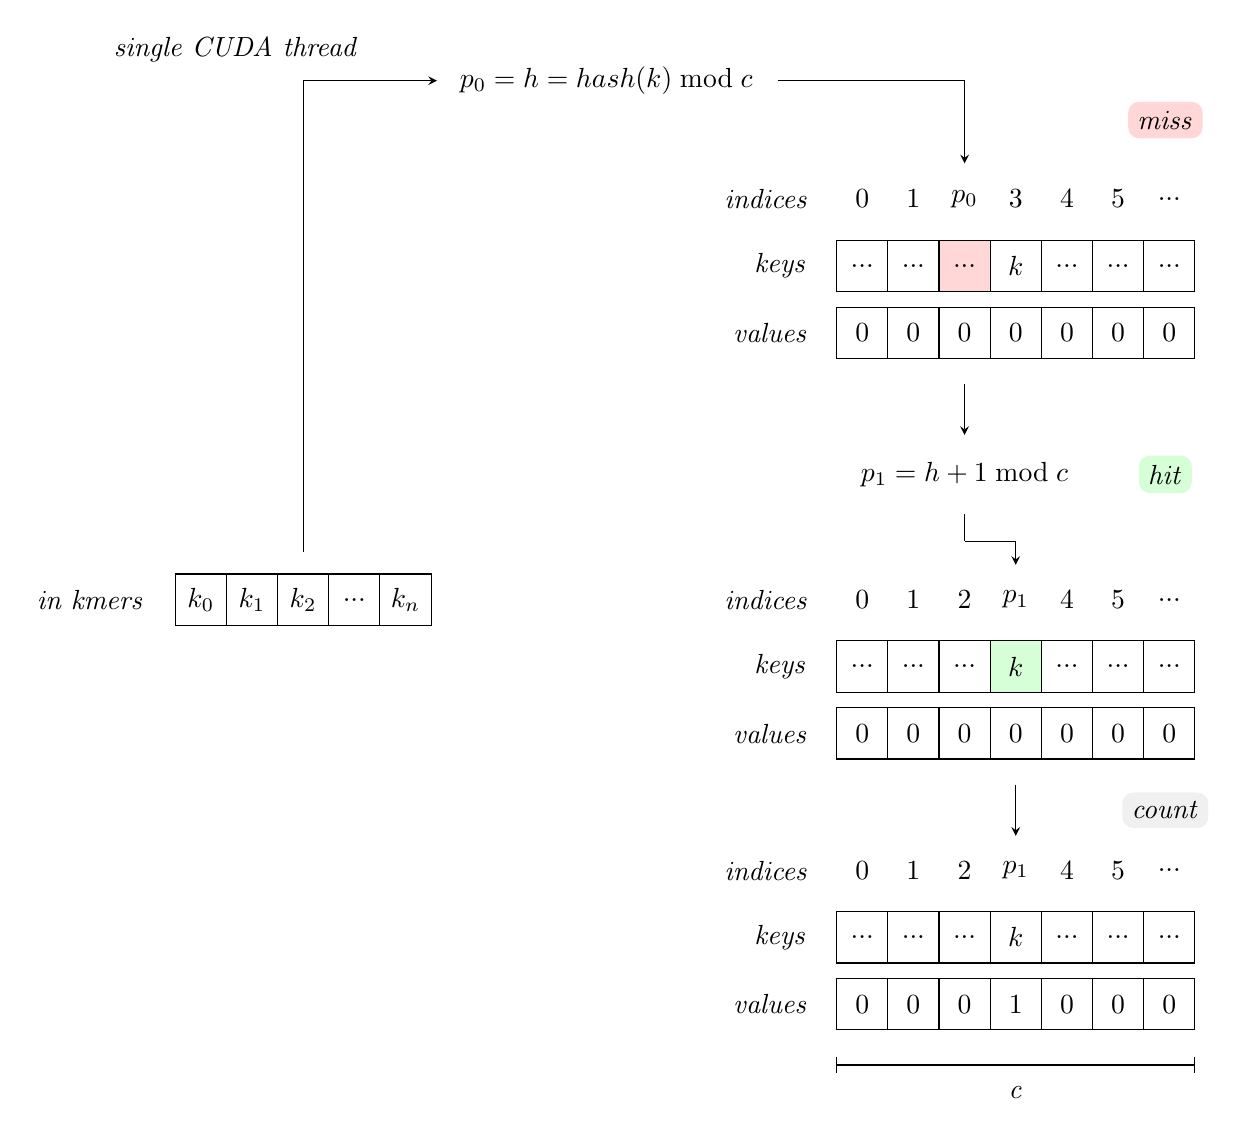
\begin{tikzpicture}

  \node at(-5.4,-7.59)(kmers){\textit{\smaller{in kmers}}};

  \node at(-4,-7.59)[draw,minimum width=0.65cm,minimum height=0.65cm](){\smaller{$k_0$}};
  \node at(-3.35,-7.59)[draw,minimum width=0.65cm,minimum height=0.65cm](){\smaller{$k_1$}};
  \node at(-2.7,-7.59)[draw,minimum width=0.65cm,minimum height=0.65cm](){\smaller{$k_2$}};
  \node at(-2.05,-7.59)[draw,minimum width=0.65cm,minimum height=0.65cm](){\smaller{$...$}};
  \node at(-1.4,-7.59)[draw,minimum width=0.65cm,minimum height=0.65cm](){\smaller{$k_n$}};

  \node at(-3.55,-0.6)[](thread){\smaller{\textit{single CUDA thread}}};
  \draw [](-2.7,-6.99) -- (-2.7,-1);
  \draw [-stealth](-2.7,-1) -- (-1,-1);

  \node at(1.15,-1)(hash){\smaller{\textit{$p_0=h=hash(k) \bmod c$}}};

  \draw [](3.325,-1) -- (5.7,-1);
  \draw [-stealth](5.7,-1) -- (5.7,-2.05);

  \node at(8.25,-1.5)[fill=misscolor,rounded corners](miss){\textit{\smaller{miss}}};

  \node at(3.185,-2.5)(indices){\textit{\smaller{indices}}};
  \node at(3.365,-3.35)(keys){\textit{\smaller{keys}}};
  \node at(3.2375,-4.2)(values){\textit{\smaller{values}}};

  \node at(4.4,-2.5)[minimum width=0.65cm,minimum height=0.65cm](){\smaller{$0$}};
  \node at(5.05,-2.5)[minimum width=0.65cm,minimum height=0.65cm](){\smaller{$1$}};
  \node at(5.7,-2.5)[minimum width=0.65cm,minimum height=0.65cm](){\smaller{$p_0$}};
  \node at(6.35,-2.5)[minimum width=0.65cm,minimum height=0.65cm](){\smaller{$3$}};
  \node at(7,-2.5)[minimum width=0.65cm,minimum height=0.65cm](){\smaller{$4$}};
  \node at(7.65,-2.5)[minimum width=0.65cm,minimum height=0.65cm](){\smaller{$5$}};
  \node at(8.3,-2.5)[minimum width=0.65cm,minimum height=0.65cm](){\smaller{$...$}};

  \node at(4.4,-3.35)[draw,minimum width=0.65cm,minimum height=0.65cm](){\smaller{$...$}};
  \node at(5.05,-3.35)[draw,minimum width=0.65cm,minimum height=0.65cm](){\smaller{$...$}};
  \node at(5.7,-3.35)[draw,minimum width=0.65cm,minimum height=0.65cm,fill=misscolor](){\smaller{$...$}};
  \node at(6.35,-3.35)[draw,minimum width=0.65cm,minimum height=0.65cm](){\smaller{$k$}};
  \node at(7,-3.35)[draw,minimum width=0.65cm,minimum height=0.65cm](){\smaller{$...$}};
  \node at(7.65,-3.35)[draw,minimum width=0.65cm,minimum height=0.65cm](){\smaller{$...$}};
  \node at(8.3,-3.35)[draw,minimum width=0.65cm,minimum height=0.65cm](){\smaller{$...$}};

  \node at(4.4,-4.2)[draw,minimum width=0.65cm,minimum height=0.65cm](){\smaller{$0$}};
  \node at(5.05,-4.2)[draw,minimum width=0.65cm,minimum height=0.65cm](){\smaller{$0$}};
  \node at(5.70,-4.2)[draw,minimum width=0.65cm,minimum height=0.65cm](){\smaller{$0$}};
  \node at(6.35,-4.2)[draw,minimum width=0.65cm,minimum height=0.65cm](){\smaller{$0$}};
  \node at(7,-4.2)[draw,minimum width=0.65cm,minimum height=0.65cm](){\smaller{$0$}};
  \node at(7.65,-4.2)[draw,minimum width=0.65cm,minimum height=0.65cm](){\smaller{$0$}};
  \node at(8.3,-4.2)[draw,minimum width=0.65cm,minimum height=0.65cm](){\smaller{$0$}};

  \draw [-stealth](5.7,-4.85) -- (5.7,-5.5);

  \node at(5.7,-6)(hash){\smaller{\textit{$p_1=h+1 \bmod c$}}};

  \draw [](5.7,-6.5) -- (5.7,-6.85);
  \draw [](5.7,-6.85) -- (6.35,-6.85);
  \draw [-stealth](6.35,-6.85) -- (6.35,-7.15);

  \node at(8.25,-6)[fill=hitcolor,rounded corners](hit){\textit{\smaller{hit}}};

  \node at(3.185,-7.59)(indices){\textit{\smaller{indices}}};
  \node at(3.365,-8.44)(keys){\textit{\smaller{keys}}};
  \node at(3.2375,-9.29)(values){\textit{\smaller{values}}};

  \node at(4.4,-7.59)[minimum width=0.65cm,minimum height=0.65cm](){\smaller{$0$}};
  \node at(5.05,-7.59)[minimum width=0.65cm,minimum height=0.65cm](){\smaller{$1$}};
  \node at(5.7,-7.59)[minimum width=0.65cm,minimum height=0.65cm](){\smaller{$2$}};
  \node at(6.35,-7.59)[minimum width=0.65cm,minimum height=0.65cm](){\smaller{$p_1$}};
  \node at(7,-7.59)[minimum width=0.65cm,minimum height=0.65cm](){\smaller{$4$}};
  \node at(7.65,-7.59)[minimum width=0.65cm,minimum height=0.65cm](){\smaller{$5$}};
  \node at(8.3,-7.59)[minimum width=0.65cm,minimum height=0.65cm](){\smaller{$...$}};

  \node at(4.4,-8.44)[draw,minimum width=0.65cm,minimum height=0.65cm](){\smaller{$...$}};
  \node at(5.05,-8.44)[draw,minimum width=0.65cm,minimum height=0.65cm](){\smaller{$...$}};
  \node at(5.7,-8.44)[draw,minimum width=0.65cm,minimum height=0.65cm](){\smaller{$...$}};
  \node at(6.35,-8.44)[draw,minimum width=0.65cm,minimum height=0.65cm,fill=hitcolor](){\smaller{$k$}};
  \node at(7,-8.44)[draw,minimum width=0.65cm,minimum height=0.65cm](){\smaller{$...$}};
  \node at(7.65,-8.44)[draw,minimum width=0.65cm,minimum height=0.65cm](){\smaller{$...$}};
  \node at(8.3,-8.44)[draw,minimum width=0.65cm,minimum height=0.65cm](){\smaller{$...$}};

  \node at(4.4,-9.29)[draw,minimum width=0.65cm,minimum height=0.65cm](){\smaller{$0$}};
  \node at(5.05,-9.29)[draw,minimum width=0.65cm,minimum height=0.65cm](){\smaller{$0$}};
  \node at(5.70,-9.29)[draw,minimum width=0.65cm,minimum height=0.65cm](){\smaller{$0$}};
  \node at(6.35,-9.29)[draw,minimum width=0.65cm,minimum height=0.65cm](){\smaller{$0$}};
  \node at(7,-9.29)[draw,minimum width=0.65cm,minimum height=0.65cm](){\smaller{$0$}};
  \node at(7.65,-9.29)[draw,minimum width=0.65cm,minimum height=0.65cm](){\smaller{$0$}};
  \node at(8.3,-9.29)[draw,minimum width=0.65cm,minimum height=0.65cm](){\smaller{$0$}};

  \draw [-stealth](6.35,-9.94) -- (6.35,-10.59);

  \node at(8.25,-10.265)[fill=countcolor,rounded corners](count){\textit{\smaller{count}}};

  \node at(3.185,-11.03)(indices){\textit{\smaller{indices}}};
  \node at(3.365,-11.88)(keys){\textit{\smaller{keys}}};
  \node at(3.2375,-12.73)(values){\textit{\smaller{values}}};

  \node at(4.4,-11.03)[minimum width=0.65cm,minimum height=0.65cm](){\smaller{$0$}};
  \node at(5.05,-11.03)[minimum width=0.65cm,minimum height=0.65cm](){\smaller{$1$}};
  \node at(5.7,-11.03)[minimum width=0.65cm,minimum height=0.65cm](){\smaller{$2$}};
  \node at(6.35,-11.03)[minimum width=0.65cm,minimum height=0.65cm](){\smaller{$p_1$}};
  \node at(7,-11.03)[minimum width=0.65cm,minimum height=0.65cm](){\smaller{$4$}};
  \node at(7.65,-11.03)[minimum width=0.65cm,minimum height=0.65cm](){\smaller{$5$}};
  \node at(8.3,-11.03)[minimum width=0.65cm,minimum height=0.65cm](){\smaller{$...$}};

  \node at(4.4,-11.88)[draw,minimum width=0.65cm,minimum height=0.65cm](){\smaller{$...$}};
  \node at(5.05,-11.88)[draw,minimum width=0.65cm,minimum height=0.65cm](){\smaller{$...$}};
  \node at(5.7,-11.88)[draw,minimum width=0.65cm,minimum height=0.65cm](){\smaller{$...$}};
  \node at(6.35,-11.88)[draw,minimum width=0.65cm,minimum height=0.65cm](){\smaller{$k$}};
  \node at(7,-11.88)[draw,minimum width=0.65cm,minimum height=0.65cm](){\smaller{$...$}};
  \node at(7.65,-11.88)[draw,minimum width=0.65cm,minimum height=0.65cm](){\smaller{$...$}};
  \node at(8.3,-11.88)[draw,minimum width=0.65cm,minimum height=0.65cm](){\smaller{$...$}};

  \node at(4.4,-12.73)[draw,minimum width=0.65cm,minimum height=0.65cm](){\smaller{$0$}};
  \node at(5.05,-12.73)[draw,minimum width=0.65cm,minimum height=0.65cm](){\smaller{$0$}};
  \node at(5.70,-12.73)[draw,minimum width=0.65cm,minimum height=0.65cm](){\smaller{$0$}};
  \node at(6.35,-12.73)[draw,minimum width=0.65cm,minimum height=0.65cm](){\smaller{$1$}};
  \node at(7,-12.73)[draw,minimum width=0.65cm,minimum height=0.65cm](){\smaller{$0$}};
  \node at(7.65,-12.73)[draw,minimum width=0.65cm,minimum height=0.65cm](){\smaller{$0$}};
  \node at(8.3,-12.73)[draw,minimum width=0.65cm,minimum height=0.65cm](){\smaller{$0$}};

  \draw [](4.075,-13.5) -- (8.625,-13.5);
  \draw [](4.075,-13.4) -- (4.075,-13.6);
  \draw [](8.625,-13.4) -- (8.625,-13.6);
  \node at(6.35,-13.85)(c){\smaller{\textit{c}}};

\end{tikzpicture}
}
\caption{As an array of 64-bit integer encoded kmers are counted by the hash table, each CUDA thread will compute the first probe position $p_0$ for each individual kmer, and then continue probing by linearly moving up to the next consecutive slot until either an empty slot or the original kmer handled by the thread is observed. If en empty slot is observed, the thread terminates. If the original kmer is observed, the value at the current slot is increased.}
\label{figure:cucounter_hashtable}
\end{center}
\end{figure}
